%!TEX root = ../main.tex

\section{The Fake News Problem}

Users today when visiting a news outlet or a social network website are commonly confronted with the question as to whether what they are reading is true or false. In this paper, we seek to assist users in tackling this problem by providing a tool to help them spot fake news.
\subsection{Current Methods to Spot Fake News}

Traditional newspapers, reputable and reliable. but fake news have been appeared precisely on such press. This has contributed to the loss of reputation of some these companies.

\mypara{Content refereeing.} To try to address this problem, some content providers have decided to employ news filtering algorithms for identifying fake news and blocking then from their users. Facebook, Twitter. Facebook has just advertised a system to classify the news based on trustworthiness~\cite{fbrank}. Facebook will begin testing the effort next week by prioritizing news reports in its news feed from publications that users have rated in Facebook surveys as trustworthy. The most ``broadly trusted'' publications—those trusted and recognized by a large cross-section of Facebook users—would get a boost in the news feed, while those that users rate low on trust would be penalized. However, we incur the risks of censorship. Recently, Twitter has been accused of blocking content from right wing circles, and from religious groups. Similar accusation has been made in 2016 to Google, Facebook, and Twitter~\cite{accusedskew}.

\mypara{Fact checkers.} To avoid this, there have appeared services specifically devoted to the identification of fake news and making them available online on some website. Examples of such services include Politifact~\cite{politifact} and FactChecker~\cite{factchecker} focused on US politics, Snopes~\cite{snopes} dedicated to urban myths, and WikiTribune~\cite{wikitribune} to global news. According to a study by the Reuters Institute~\cite{risefackchecking}, in 2016 there were nearly 113 organizations dedicated to fact checking, 90\% of them created since 2010. A fake news organization has even been formed just for this effect, and campaigns for educating users to help them spot fake news. However, the way these systems are build is decoupled from the websites they see, which makes it harder to spot fake news as they visit their preferred news providers. Furthermore, it is sometimes hard for end-users to assess how trustworthy such sources are, making it difficult for users to determine the provenance of the information and reliability of the fact checker. It is sometimes the case that the sources of information are narrowed to specific domains. Another type of system is the Wikipedia, which has already moderation, but relies on a centralized silo of information, with no way for end-users to be able to validate the original provenance of the information.

\mypara{Automatic detection.} There are also emerging automated systems for classifying. But the problem is how to really assess if the results correspond to the truth? It may end up being something where democracy counts. On the other hand it may be possible to build a system where the source of data is already trustworthy and what the system does is to check it. However this is not going to work for real world news where facts have to be validated against external sources before they can be deemed trustworthy. Some previous studies aimed to detect deceptive text on crowdsourced datasets using various techniques, such as stylometric~\cite{stylometric}, semi-supervised learning~\cite{semisupervised}, and linguistic approaches~\cite{linguistic}. Liar~\cite{liar}.

%Centralized solution for someone who stores everything and validates that information for you. Problem of facebook, twitter being accused of bias.

\subsection{New Approach: Distributed Verifiable Claims}


\begin{figure}[t]
  \centering
  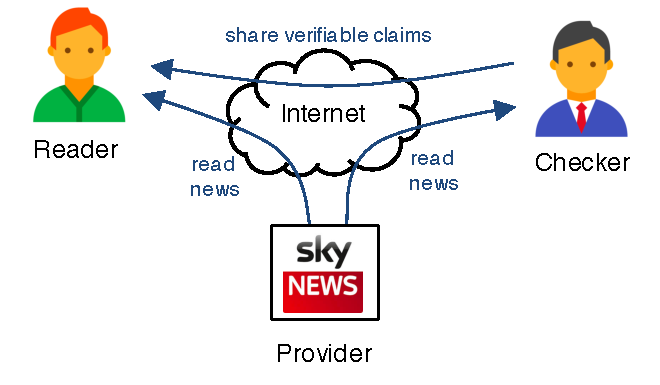
\includegraphics[width=0.9\columnwidth]{figures/model.pdf}
  \vspace{-10pt}
  \caption{Fake news detection based on verifiable claims.}
%  \vspace{-0.3cm}
  \label{fig:model}
\end{figure}

Verifiable Claims are a proposal by W3C. Our data model, Distributed Verifiable Claims are based on W3C's verifiable claims but with some differences.

\subsubsection{Verifiable Claims Data Model}
Verifiable Claims are a data representation modal, proposed by the W3C Credentials Community Group \footnote{https://web.archive.org/web/20171013165205/https://www.w3.org/TR/verifiable-claims-data-model/} for describing achievements, qualities or other information.

An example would be a university digital diploma, singed by the university’s private key, that I can take to any employer and they can verify it. This diploma should continue to be verifiable even if the university ceases to exist.

Actions supported by Verifiable Claims:
\begin{itemize}
    \item Issue
    \item Share / retrieve
    \item Verify
    \item Revoke
\end{itemize}


What we want to do is to provide a platform that allows end users to have news items automatically reviewed by independent parties of their trust. News are understood as claims which are submitted to a review process. Figure~\ref{fig:model} shows how we envision it working. In our system there are three parties: providers, readers, and issuers. Providers are responsible for serving news content to the users on their browsers. Readers are nothing but the end users which visit providers' websites and browse through the news content. Issuers are responsible for reviewing certain news and issuing a certificate which will be associated to the news.

The idea is that the readers are able to check if some news items is reliable or fake depending on the endorsement produced by some issuer. Readers should be able to designate which issuers they trust so that by the time they visit a given website, each news item is classified according to the review generated by the issuer.

Note that it is not our goal to build a tool that can determine {\em per se} and automatically fake news. Our approach is instead to let readers establish trust relations with someone that they trust to provide them with reliable information. This can be, e.g., some original author, communities of experts, etc. Our system should allow issuers also to attach proofs of what they say is true. Put simply, we want to provide an instrument that can help news readers to mimic trust relations they have in the real world also in the virtual world.


\subsection{Challenges}

In order to build a system for fake news detection based on verifiable claims, several challenges need to be overcome:

\mypara{Censorship resistance:} How to prevent someone from blocking access to the content or preventing issuers from submitting their reviews to the system.

\mypara{Security:} How to ensure that the news are not altered, that the content is not modified, and that it is possible for users to be sure that a certain given content has been endorsed by someone they really trust.

\mypara{Resilience:} We need to ensure that our system survives attacks from powerful organizations and is able to preserve the content persistently for a long time span.

\mypara{Source anonymity:} How to provide anonymity protection? Talk about privacy. 

\mypara{Incentives} Talk about incentives that must be aligned. Talk about sustainability.


